% Titre de la premiere partie
\section[]{Introduction \& Motivation}

%%%%%%%%%%%%%%%%%%%%%%%%%%%%%%%%%%%%%%%%%%%%%%%%
% Première diapo
%%%%%%%%%%%%%%%%%%%%%%%%%%%%%%%%%%%%%%%%%%%%%%%%
\begin{frame}
\frametitle{Introduction \& Motivation}
\framesubtitle{Toric Symplectic Manifolds}

\begin{defn}
	$(X^{2n}, \w)$ is a \emph{toric symplectic manifold} if it is compact, connected, and equipped with an effective hamiltonian action of $T^{n}$, with moment map $\mu:X \rightarrow (\RR^{n})^{\ast}$.
\end{defn}

\begin{ex}
	$(\CC\PP^{2}, \w_{FS})$, with $T^{2}$-action given by:
	$$
		(t_{1},t_{2})\cdot [z_{0}: z_{1}: z_{2}] = [z_{0}: t_{1}z_{1}: t_{2}z_{2}].
	$$
	Moment map $\mu:\CC\PP^{2} \rightarrow (\RR^{2})^{\ast}$ is:
	$$
		\mu([z_{0}:z_{1}:z_{2}]) = \frac{1}{2}\bigg( \frac{|z_{1}|^{2}}{\|z\|^{2}}, \frac{|z_{2}|^{2}}{\|z\|^{2}}   \bigg) + c,\qquad c \in (\RR^{2})^{\ast}.
	$$
\end{ex}

\end{frame}


%%%%%%%%%%%%%%%%%%%%%%%%%%%%%%%%%%%%%%%%%%%%%%%%
% Deuxième diapo
%%%%%%%%%%%%%%%%%%%%%%%%%%%%%%%%%%%%%%%%%%%%%%%%
\begin{frame}
\frametitle{Introduction \& Motivation}
\framesubtitle{Delzant Polytopes}

\begin{defn}
	$\Delta \subset (\RR^{n})^{\ast}$ is a \emph{Delzant polytope} if it is convex, simple, rational and smooth.
\end{defn}

\begin{exs}
	\begin{figure}
		\centering
		$\CC\PP^{2}\leftrightarrow$\hspace{-24pt}
		\begin{minipage}{.3\textwidth}
			\centering
			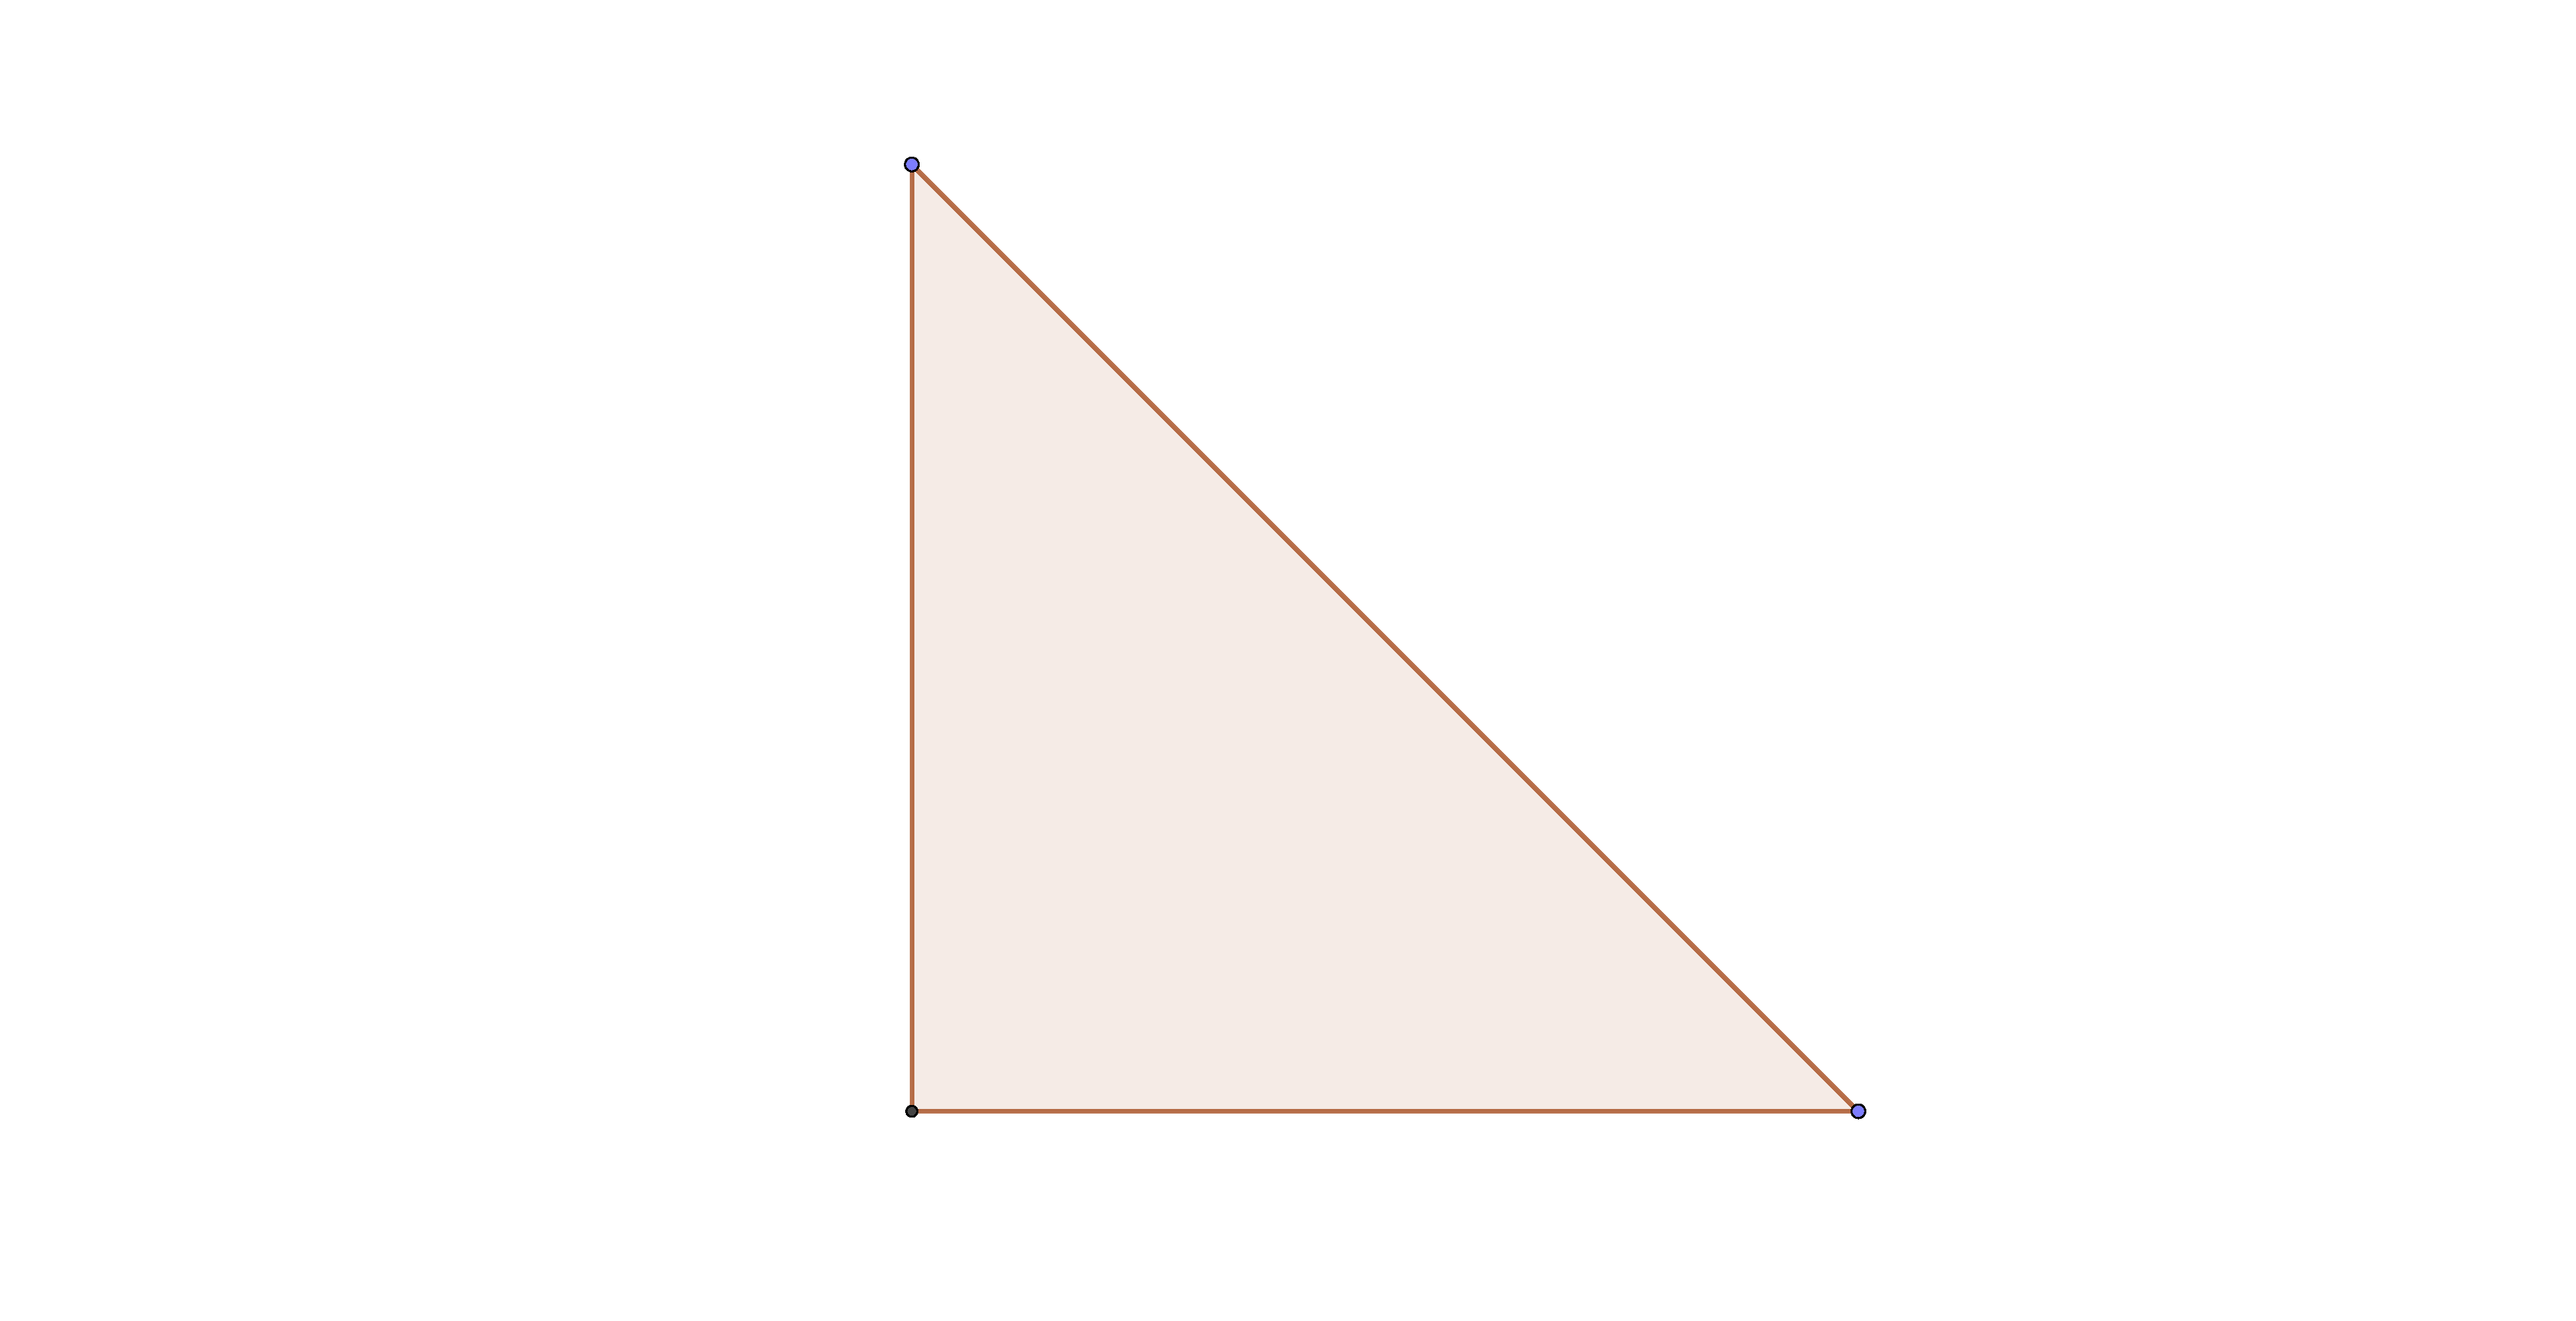
\includegraphics[width=.4\linewidth]{figures/cp2-polytope}
		\end{minipage}%
		\begin{minipage}{.3\textwidth}
			\centering
			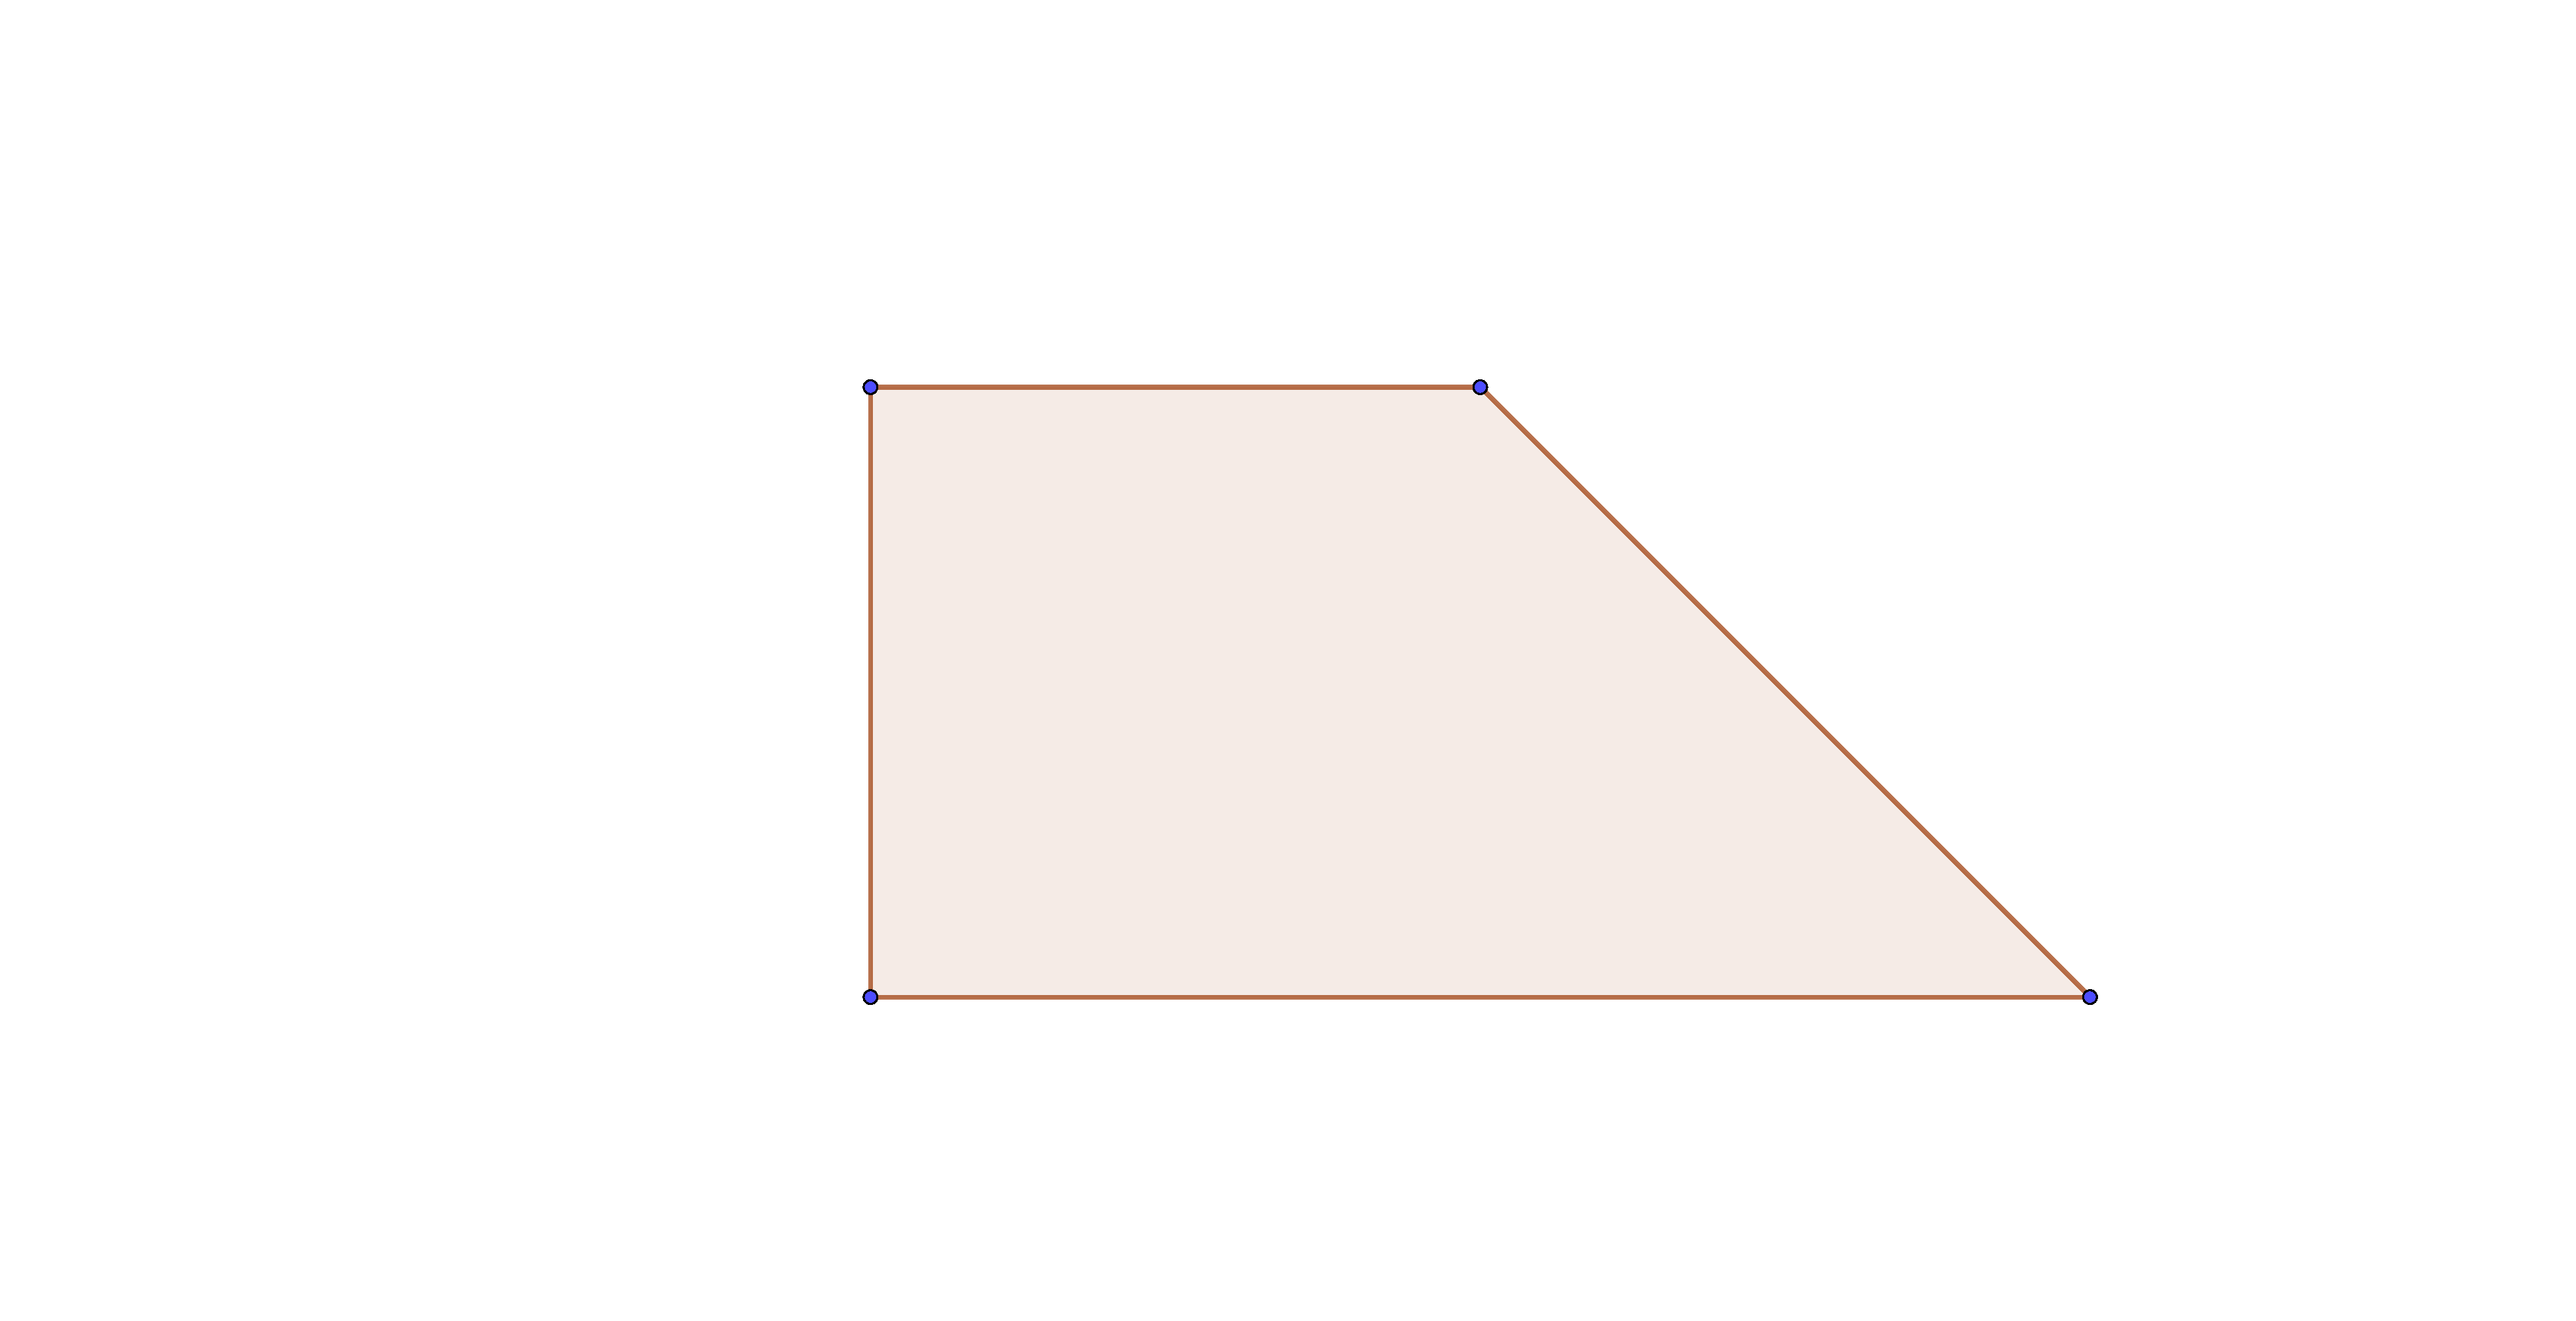
\includegraphics[height=.4\linewidth]{figures/blowup-polytope}
		\end{minipage}
		\hspace{-12pt}$\leftrightarrow$\ \reallywidetilde{\CC\PP^{2}}
	\end{figure}
\end{exs}

\end{frame}

%%%%%%%%%%%%%%%%%%%%%%%%%%%%%%%%%%%%%%%%%%%%%%%%
% Troisième diapo
%%%%%%%%%%%%%%%%%%%%%%%%%%%%%%%%%%%%%%%%%%%%%%%%
\begin{frame}
	\frametitle{Introduction \& Motivation}
	\framesubtitle{Delzant Construction}
	
	\begin{rmk}
		Given $(X^{2n}, \w, T^{n}, \mu)$, the Atiyah, Guillemin-Sternberg convexity theorem asserts that $\mu(X^{2n}) = \Delta \subset (\RR^{n})^{\ast}$ is a Delzant polytope.
	\end{rmk}
	
	\begin{thm}[Delzant]
		$$
		\frac{(X^{2n}, \w,T^{n},\mu)}{T^{n}\text{-equivariance}} \overset{1-1}{\longleftrightarrow} \frac{\text{Delzant polytopes}}{SL(n,\ZZ) \ltimes \RR^{n}}
		$$
	\end{thm}
	
	\begin{qstn}
		So for a given $\Delta \subset (\RR^{d})^{\ast}$, what is the respective $X_{\Delta}$?
	\end{qstn}


\end{frame}

%%%%%%%%%%%%%%%%%%%%%%%%%%%%%%%%%%%%%%%%%%%%%%%%
% Troisième diapo
%%%%%%%%%%%%%%%%%%%%%%%%%%%%%%%%%%%%%%%%%%%%%%%%
\begin{frame}
	\frametitle{Introduction \& Motivation}
	\framesubtitle{Delzant Construction}
	
	Let $u_{i}\in \RR^{d}$ $(i=1,\ldots,n)$ be the inward-pointing normals to to facets of $\Delta$, and define $\pi(e_{i}) = u_{i}$.
	
	\begin{equation*}
	\begin{tikzcd}[ampersand replacement=\&]
	0 \arrow[r] \& \mf{n}:= \ker \pi \arrow[r, "i",hook] \& \mathbb{R}^{n} \arrow[r, "\pi"] \& \mathbb{R}^{d} \arrow[r] \& 0
	\end{tikzcd}
	\end{equation*}
	Can dualise:
	\begin{equation*}
	\begin{tikzcd}[ampersand replacement=\&]
	0 \& \arrow[l] \mf{n}^{\ast} \& \arrow[l, "i^{\ast}",swap] (\mathbb{R}^{n})^{\ast} \& \arrow[l,"\pi^{\ast}",swap] (\RR^{d})^{\ast} \& \arrow[l] 0
	\end{tikzcd}
	\end{equation*}
	Or exponentiate:
	\begin{equation*}
	\begin{tikzcd}[ampersand replacement=\&]
	0 \arrow[r] \& N \arrow[r, "i",hook] \& T^{n} \arrow[r, "\pi"] \& T^{d} \arrow[r] \& 0
	\end{tikzcd}
	\end{equation*}
	
\end{frame}

%%%%%%%%%%%%%%%%%%%%%%%%%%%%%%%%%%%%%%%%%%%%%%%%
% Troisième diapo
%%%%%%%%%%%%%%%%%%%%%%%%%%%%%%%%%%%%%%%%%%%%%%%%
\begin{frame}
	\frametitle{Introduction \& Motivation}
	\framesubtitle{Delzant Construction}
	
	\begin{equation*}
	\begin{tikzcd}[ampersand replacement=\&]
	0 \arrow[r] \& N \arrow[r, "i",hook] \& T^{n} \arrow[r, "\pi"] \& T^{d} \arrow[r] \& 0
	\end{tikzcd}
	\end{equation*}
	
	$T^{n}$ acts diagonally on $\CC^{n}$, with moment map:
	$$
		J:\CC^{n} \rightarrow (\RR^{n})^{\ast},\qquad J(z) = \frac{1}{2}\sum_{i=1}^{n}(|z_{i}|^{2} - \lambda_{i})e_{i},\quad \lambda\in (\RR^{n})^{\ast}.
	$$
	$N$ also acts on $\CC^{n}$ via inclusion, with moment map $i^{\ast}\circ J: \CC^{n} \rightarrow \mf{n}^{\ast}$.
	
	
	\begin{fact}
		$X_{\Delta} := (i^{\ast}\circ J)^{-1}(0) / N$ is a toric symplectic manifold for the residual $T^{d}$-action, with Delzant polytope $\Delta$, where $$\Delta = \cap_{i=1}^{n} \{y \in \RR^{d} \st \langle y, u_{i} \rangle \geq \lambda_{i} \text{ for all } i  \}.$$
	\end{fact}
	
\end{frame}


%%%%%%%%%%%%%%%%%%%%%%%%%%%%%%%%%%%%%%%%%%%%%%%%
% Troisième diapo
%%%%%%%%%%%%%%%%%%%%%%%%%%%%%%%%%%%%%%%%%%%%%%%%
\begin{frame}
\frametitle{Introduction \& Motivation}
\framesubtitle{Geometric Quantisation}

\begin{qstn}
	For a (pre-quantum) line bundle $\mc{L}$ over $(X,\w)$, can one find a canonical Hilbert space of (holomorphic) ``wave-functions'' $\mc{Q}(X)$ with 
	$$
		\mc{Q}(X) = H^{0}(X,\mc{L})?
	$$
\end{qstn}

\begin{conj}[``Quantisation Commutes with Reduction'']
	If $X_{0} = \mu^{-1}(0)/G$, then:
	$$
		\mc{Q}(X)^{G} = \mc{Q}(X_{0})
	$$
	Further, if $X_{\alpha} = \mu^{-1}(\alpha)/G$:
	$$
		\dim \mc{Q}(X_{\alpha}) = \mult(\alpha)
	$$
\end{conj}

\end{frame}


%%%%%%%%%%%%%%%%%%%%%%%%%%%%%%%%%%%%%%%%%%%%%%%%
% Troisième diapo
%%%%%%%%%%%%%%%%%%%%%%%%%%%%%%%%%%%%%%%%%%%%%%%%
\begin{frame}
	\frametitle{Introduction \& Motivation}
	\framesubtitle{Lattice Point Counting}
	
	\begin{thm}
	For toric symplectic manifolds:
	$
		\dim \mc{Q}(X) = \#(\Delta \cap \ZZ^{n})
	$
	\end{thm}

	\begin{ex}
		$X = \CC^{3}$ and $\CC\PP^{2} = X_{k} = \mu^{-1}(k)/N$. For $s:\CC^{3} \rightarrow \CC$ holomorphic, locally $s(z) = z_{0}^{j_{0}}z_{1}^{j_{1}}z_{2}^{j_{2}}$. For $N$-equivariance:
		\vspace{-10pt}
		$$
			s(n\cdot z) = n^{j_{0} + j_{1} + j_{2}}s(z) \overset{?}{=} n\cdot s(z) = n^{k}s(z).
		$$
		True for $H^{0}(\CC\PP^{2},\mc{O}(k))$, and solution set:
		$$
			\{(j_{0}, j_{1}, j_{2}) \st \sum j_{i} = k  \} \overset{1-1}{\leftrightarrow} \{(j_{0}, j_{2})\st j_{0} + j_{1} \leq k  \} \equiv (\Delta \cap \ZZ^{2}).
		$$
	\end{ex}

\end{frame}

%%%%%%%%%%%%%%%%%%%%%%%%%%%%%%%%%%%%%%%%%%%%%%%%
% Troisième diapo
%%%%%%%%%%%%%%%%%%%%%%%%%%%%%%%%%%%%%%%%%%%%%%%%
\begin{frame}
		\frametitle{Introduction \& Motivation}
		\framesubtitle{The Verlinde Formula}
		
	\begin{rmk}
		Case for $X = \CC^{4}$ and $X_{k} = \mu^{-1}(k)/N \cong \CC\PP^{3}$ very similar, with Delzant polytope $k\Delta \subset \RR^{3}$ ($\Delta$ the standard $3$-simplex).
		$$
		\#(k\Delta \cap \ZZ^{3}) = \frac{(k+1)(k+2)(k+3)}{3!} = \frac{k^{3}}{6} + k^{2} + \frac{11}{6}k + 1.
		$$
	\end{rmk}

	\begin{fact}
		Let $M = \mc{M}_{\text{flat}}(\Sigma_{2};SU(2))$, and $\mc{L}$ be the determinant line bundle. Then:
		$$
			\dim H^{0}(M,\mc{L}^{\otimes k}) = \#(k\Delta \cap \ZZ^{3}).
		$$
		In fact, $M \cong \CC\PP^{3}$, and the above equation is known as the \emph{Verlinde formula} for $M$.
	\end{fact}	

\end{frame}

%%%%%%%%%%%%%%%%%%%%%%%%%%%%%%%%%%%%%%%%%%%%%%%%
% Troisième diapo
%%%%%%%%%%%%%%%%%%%%%%%%%%%%%%%%%%%%%%%%%%%%%%%%
\begin{frame}
	\frametitle{Introduction \& Motivation}
	\framesubtitle{Higgs Bundle Moduli}
	
	\begin{qstn}
		What about the moduli space for Higgs bundle $\mc{M}_{\text{Higgs}}(\Sigma_{g};G)$, which is \emph{non-compact}?
	\end{qstn}

	It has $T^{\ast}\mc{M}_{\text{flat}}(\Sigma_{g};G) \subset \mc{M}_{\text{Higgs}}(\Sigma_{g};G)$ as an open and dense subset.
	As $\mc{M}_{\text{Higgs}}$ is non-compact, $\dim \mc{Q}(\mc{M}_{H}) = \infty$.
	However $\mc{M}_{H}$ admits a $\CC^{\ast}$-action by scaling the Higgs fields, and $S^{1}\subset \CC^{\ast}$ has compact fixed point loci $\implies \CC^{\ast}$-weight decomposition:
	$$
	\mc{Q}(\mc{M}_{H}) = \bigoplus_{n\geq 0}\mc{Q}(\mc{M}_{H})_{n}.
	$$
	
\end{frame}

%%%%%%%%%%%%%%%%%%%%%%%%%%%%%%%%%%%%%%%%%%%%%%%%
% Troisième diapo
%%%%%%%%%%%%%%%%%%%%%%%%%%%%%%%%%%%%%%%%%%%%%%%%
\begin{frame}
	\frametitle{Introduction \& Motivation}
	\framesubtitle{The Equivariant Verlinde Formula}

	\begin{prop}
		The \emph{equivariant Verlinde formula} is a recipe for calculating the $n$\textsuperscript{th} graded part for $\dim \mc{Q}(\mc{M}_{\text{Higgs}})$, \ie 
		$$
			\dim_{t} H^{0}(\mc{M}_{H},\mc{L}^{k}) = \sum_{n=0}^{\infty}\dim H_{n}^{0}(\mc{M}_{H},\mc{L}^{k})t^{n}.
		$$
		\end{prop}	
	In particular, the degree-0 (weight-0) part corresponds to the classical Verlinde formula.
	
	\begin{rmk}
		There is also an equivariant Verlinde formula for \emph{parabolic Higgs bundles}.
	\end{rmk}
\end{frame}